\section{Project Analysis} \label{analysis}

\subsection{A Brief Introduction to Fractals}

A fractal is ``a curve or geometrical figure, each part of which has the same statistical character as the whole''\cite{soanes_hawker_2013}.

Some fractals are defined by simple equations which exhibit chaotic behaviour. Arguably the most famous fractal, the Mandelbrot Set, is defined by the following iterative equation, where \(Z_0=0+0i\) and \(C\) is the initial value in the complex plane.

\begin{equation}
	Z_{n+1} = Z_n^2 + C \quad:\quad Z_n, c \in \mathbb{C}		
\end{equation}

For a given point \(C\) to be in the Mandelbrot Set, the value of \(Z_n\) must remain bounded (i.e. not diverge to infinity) after the iterative series is repeated infinitely many times. This approach is used in most iterative fractal equations.

\vspace{0.5cm}

\begin{figure}[h]
    \centering
	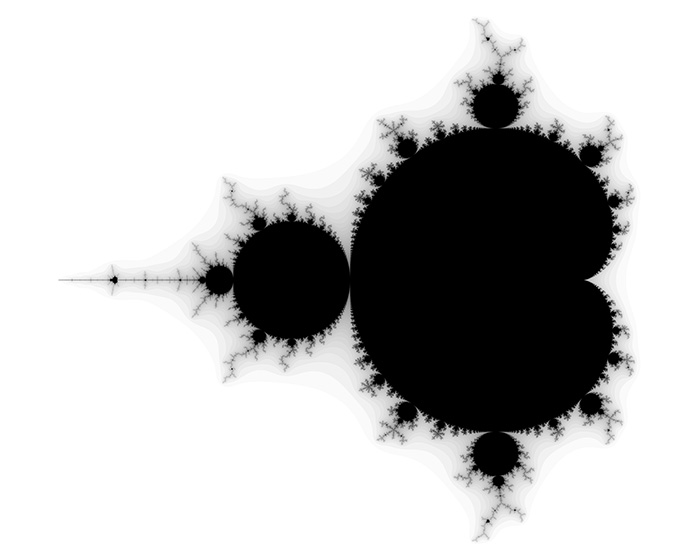
\includegraphics[scale=0.45]{mandelbrot.jpg}
	\caption{The standard Mandelbrot fractal\cite{bourke_2002}}
\end{figure}

Additionally, fractal variations can be created by changing the generating equation slightly. For example, changing the \(r\) in the Mandelbrot equation (\(Z_{n+1}=Z_n^r+C\)) yields the following fractals.

\begin{figure} [htp]
	\centering
	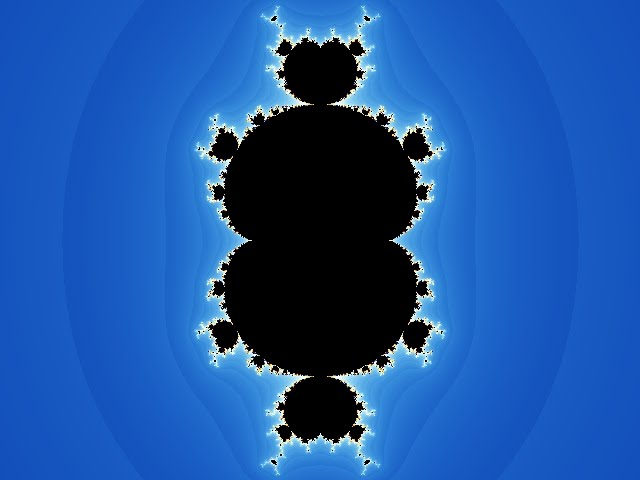
\includegraphics[width=.3\textwidth]{MsetOrder3.jpg}\hfill
	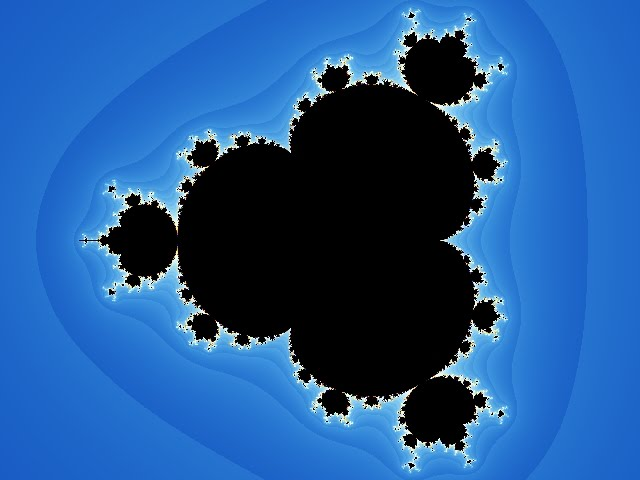
\includegraphics[width=.3\textwidth]{MsetOrder4.jpg}\hfill
	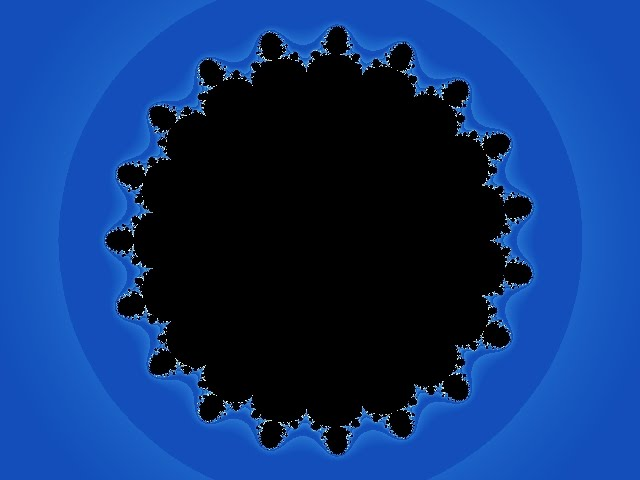
\includegraphics[width=.3\textwidth]{MsetOrder20.jpg}
	
	\caption{(left) \(r=3\), (centre) \(r=4\), (right) \(r=20\)}
\end{figure}

Other famous fractals include the Sierpiński Triangle, the Julia Set, Hilbert Spirals, etc. All are defined either by infinitely-recursive self-similar patterns or repeated equations.

\begin{figure}[htp]
	\centering
	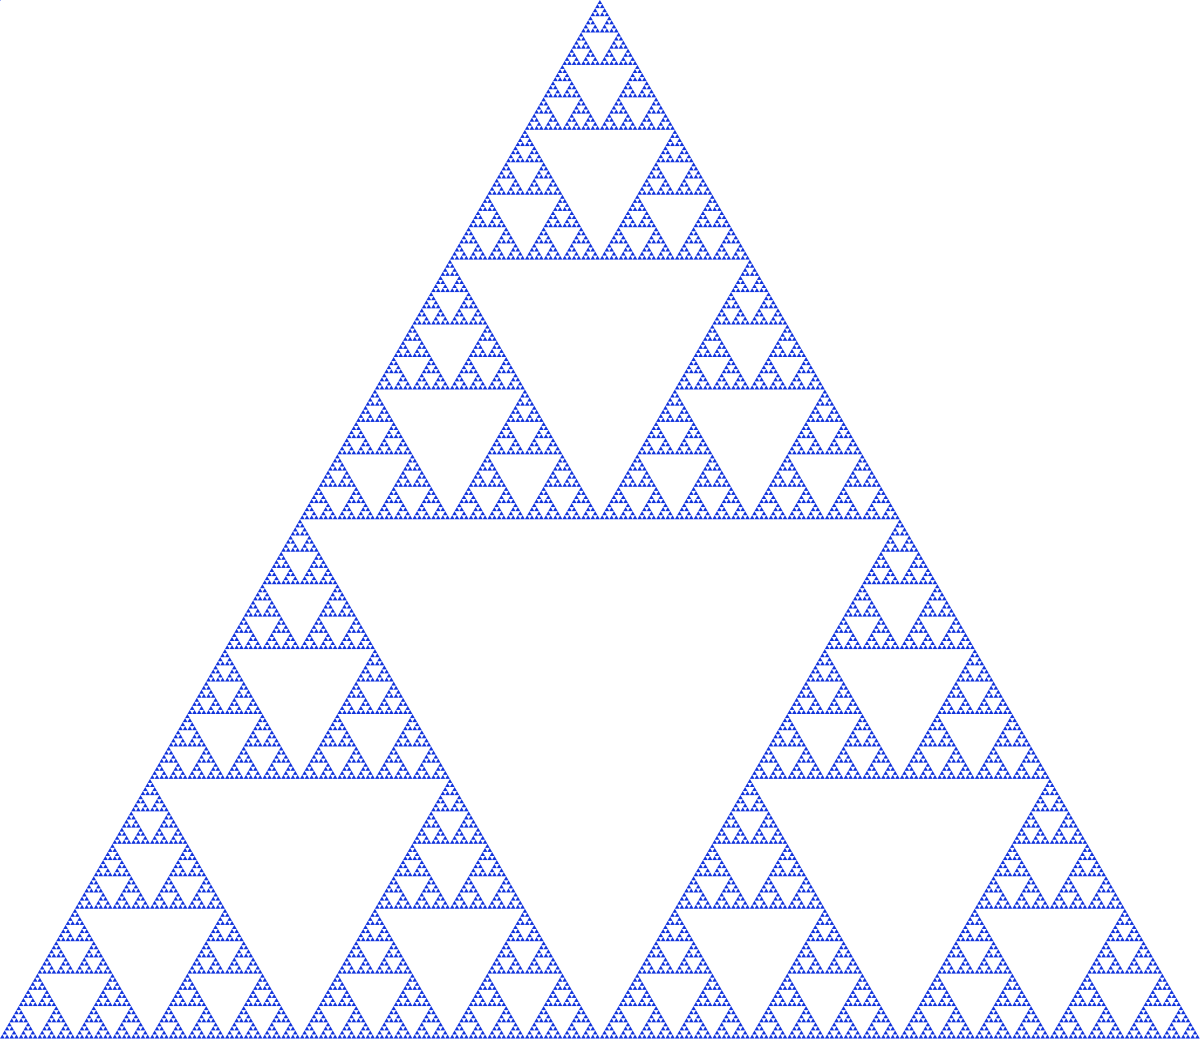
\includegraphics[width=.3\textwidth]{sierpinski-triangle.png}\hfill
	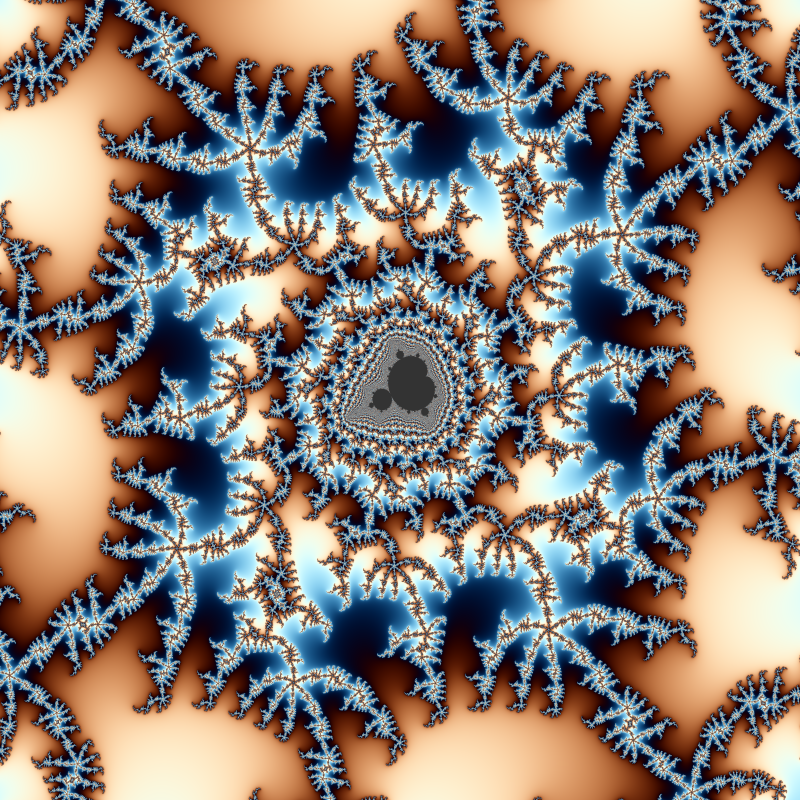
\includegraphics[width=.3\textwidth]{mandelbrot-zoom.png}\hfill
	
\includegraphics[width=.3\textwidth]{hilbert-curve.png}
	
	\caption{(left) Sierpiński-Triangle, (centre) Part of the Mandelbrot Set, (right) Hilbert Curve}
\end{figure}

\subsection{Defining the Problem}

Fractals have been the subject of much debate and curiosity throughout history. However, due to the computational requirements of generating them, research into them was minimal until the rise of the electronic computer.

The newfound processing power allowed increasingly detailed images to be generated, and mathematicians could better understand fractals' underlying equations and seemingly chaotic nature.

With the power of modern computers, it is possible to render some fractals in real-time and explore them to great depths, though there are still technical, physical and monetary hurdles to clear.

Many fractal rendering programs exist online; however, most are incomplete, inefficient applications not designed for high performance and increased zoom factors. While many high-quality applications exist, the best ones are often quite expensive, making them inaccessible to most potential users. For example, some extremely advanced software costs almost \(\pounds 80\)\cite{slijkerman_2022}.
	
\paragraph{Technological Limitations} The further you zoom into a fractal, the smaller the numbers you have to deal with. At lower zoom levels, this doesn't pose much of an issue, as \SI{64}{\bit} or even \SI{32}{\bit} floating point numbers often have the required precision to render an image accurately. At higher zoom levels, however, the precision of the numbers used affects the image quality.

When zoomed in far enough, floating point rounding errors start to cause certain pixel positions to merge into one, causing unattractive ``blocky'' patterns in the image. Eventually, these blocks will consume the entire image, and no more detail can be seen.

To get around this, it is possible to use high-precision floating point data types. However, since these are processed in software, not hardware, they are orders of magnitude slower than normal number types, which can make the rendering process impractically slow.

Some techniques can be taken to optimise the performance of high-performance number types. For example, it can be proven that \(Z_n\) will diverge to infinity if \(|Z_n|>2\) at any point. Additionally, advanced algorithms can mix fixed and multi-precision arithmetic to decrease the number of operations performed in software.

\paragraph{Program Limitations} Many fractal renderers do just that; render fractals. They don't support any render export features and do not allow for saving, reloading or sharing render configurations. 

Some programs have methods to save the rendered fractals as image files but often have limiting export settings and don't support many resolutions. Some programs allow the current position and zoom level, among other information, to be exported to a file, allowing interesting fractal locations to be shared easily.

\paragraph{Precision vs Performance} To increase rendering performance, most implementations of fractal renderers use 32- or 64-bit floating point numbers. Since operations on these data types are performed directly by hardware, they are highly efficient. Unfortunately, 64-bit floating point values can only accurately represent around 15 decimal places, so zooming in far enough will exceed this precision and cause visual glitches.

To circumvent this issue, it is possible to use multi-precision floating point types capable of representing hundreds, thousands or even millions of bits, allowing for near-infinite zooms. These numbers, however, are implemented in software and are many orders of magnitude slower than standard floating point types. It is possible to use multi-precision floating point arithmetic for sufficiently optimised programs, though the performance will be abysmal.

Furthermore, some areas of different fractals require a considerable number of iterations before a reasonable amount of detail can be obtained. As a result, potentially millions of calculations must be done to determine the colour for a single pixel.

The two main issues above become even more extreme when combined with the goal of near-infinite zooming. Due to the nature of many fractals, the number of iterations required to get high levels of detail in areas close to the border of the fractal increases with zoom. Additionally, deeper zooms need higher precision numbers to represent all the points accurately. Combine these, and the result is a slow, inefficient program.

\subsection{The End User}

\vspace{0.25cm}
\noindent
\textbf{Mathematics Teachers and Professors} could use the program to assist in their lessons and provide students with an interactive resource to help with homework and further their understanding. This could dramatically increase students' engagement in studies and inspire them to pursue further degrees in mathematics. Additionally, less well-off schools could afford and use the software if the program is free and open source, increasing its accessibility.

\vspace{0.25cm}
\noindent
\textbf{Researchers and General Acedmia} could use the high precision, deep zooms and fast renders to further their studies on the properties of fractals. Furthermore, the more advanced fractal export tools could be used to share the exact configurations of the areas they explore to accelerate the peer-review process.

\vspace{0.25cm}
\noindent
\textbf{Anyone Interested in Mathematics} could explore fractals' beauty and share the rendered images with their friends and family. If the program is suitably intuitive, even young children would be able to use it, potentially inspiring an interest in mathematics.

\subsection{Analysis of Existing Programs}

\subsubsection{David J. Eck's Online Mandelbrot Renderer \cite{eck}}

David Eck's online Mandelbrot rendering program implements many nice-to-have features, including the ability to export the current render settings as an XML file, intuitive controls and various configuration settings. The user can easily change the colour palette, image resolution, the number of threads to use, and more.

This implementation also supports a multi-precision floating point type, which allows the renderer to zoom in ``infinitely''. Unfortunately, this renderer is written in Javascript rather than a faster language like Java or, better yet, \CPP; as a result, it can take a long time to render an image, especially at higher resolutions and quality settings.

\vspace{0.25cm}

\paragraph{Interface} The interface for this renderer is quite primitive and, while intuitive, is not pleasant to use. The box select to zoom in can be frustrating to use and often results in poor framing since it zooms in immediately after releasing the mouse.

The status indicator shows the current render progress and is extremely limited. It shows the current pass of the renderer, the precision it is using and the number of rows completed, but there is nothing showing the estimated time remaining, the speed at which it is rendering, or the time elapsed since the render started.

\paragraph{Configuration} While the renderer allows for the major settings to be changed, such as the maximum number of iterations to perform, the colour palette and the number of threads to use, many of the more advanced settings cannot be changed. For advanced applications, it is often useful to know \textit{exactly} where the frame is centred in fractal space. An arguably more important feature is the ability to specify a location and scaling factor directly, instead of zooming in manually.

On the other hand, the ability to revert to default settings, combined with the lists of predefined settings for each option, make the program much more accessible for the less experienced. This feature is a must-have for a program aimed at a wide audience.

\paragraph{Render Quality} While the user can specify the resolution at which to render the image, it must fit on the screen you are using. You cannot render a higher-resolution image to a file, for example. Furthermore, there are no options to configure anti-aliasing with this renderer, which means the image quality may not be as high as required for some purposes.

\subsubsection{XaoS.js Online Mandelbrot Renderer \cite{xaos.js}}

The Fractal Foundation \textit{XaoS.js} Mandelbrot renderer is relatively primitive, using only machine-precision floating point arithmetic and no options to configure the fractal. On the other hand, the renderer is intuitive, with a simple click-to-zoom interface, making it ideal for less knowledgeable users who want to explore fractals.

However, the \textit{XaoS.js} renderer does implement some complex rendering algorithms. It maintains existing pixel information from the previous frame and uses it to refine the next one, creating a smoother transition progressively. Unfortunately, these rendering techniques result in significant artefacts when sufficiently zoomed in (though the limited number of iterations performed means the fractal is unrecognisable at this point).

\subsubsection{XaoS Offline Fractal Renderer \cite{fractalfoundation}}

The Fractal Foundation \textit{XaoS} fractal renderer is a much more advanced, offline version of the previously examined program. Since it is free and open-source, many people have contributed code and developed its rendering algorithms. As a result, it can render fractals much faster than other programs. However, the advanced techniques used cause artefacts to appear in the final renders, making it unsuitable for academic or research purposes since it is not a true likeness of the fractal.

\FloatBarrier

\begin{figure}[htp]
    \centering
    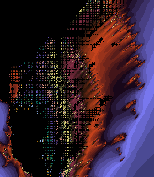
\includegraphics[width=0.3\textwidth]{xaosArtefacting0.png}
    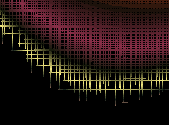
\includegraphics[width=0.4655\textwidth]{xaosArtefacting1.png}
    \caption{Artefacting in the XaoS renderer}
\end{figure}

\FloatBarrier

\paragraph{Interface} \textit{XaoS} has the same intuitive controls as the online implementation, but all the configuration options are hidden in awkward menus at the top of the screen.

\paragraph{Configuration} With enough searching, almost every parameter about the fractal can be changed, including filters such as edge detection and anti-aliasing. This is incredibly useful for advanced users, as it enables them to adjust the appearance of the fractal to their exact needs, emphasising the features they are investigating.

\paragraph{File Export} \textit{XaoS} allows the user to export a configuration file or save the current render as an image. The configuration file contains the information required to reconstruct the image in the renderer, simplifying the sharing of fractals between users. The image export saves the current pixels of the screen to a file, meaning the image's resolution is limited to the size of the window. This is unfortunate for those who may want to save a high-resolution image but cannot make the window large enough to support this.

\FloatBarrier
\begin{figure}[htp]
    \centering
    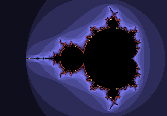
\includegraphics[scale=1.5]{xaosImage.png}
    \caption{A low-quality image saved from XaoS}
\end{figure}
\FloatBarrier

\paragraph{Supported Fractals} The \textit{XaoS} renderer supports 25 common fractals by default and can render simple user-defined fractals. While nice to have, this feature is unnecessary for a program to implement, assuming it supports at least two fractal types. Additionally, the user-defined fractals tend to render much slower than the built-in ones since optimised algorithms can be developed for them.

\paragraph{Precision} \textit{XaoS} uses fixed-precision arithmetic to perform calculations; hence, you cannot zoom into the fractals indefinitely. Given the performant nature of the program, it is unfortunate that this is not a feature since it could outcompete most other rendering programs.

\subsection{Program Requirements}

\begin{enumerate}
    \item Rendering \label{req_rendering}
    \item Configuration \label{req_configuration}
    \item Interface and Movement \label{req_interface}
    \item Import and Export \label{req_import_export}
    \item Installation \label{req_install}
    \item Performance \label{req_performance}
\end{enumerate}


\newcommand{\highPriority}[0]{{\color{red} \textbf{HIGH}}}
\newcommand{\mediumPriority}[0]{{\color{orange} \textbf{MEDIUM}}}
\newcommand{\lowPriority}[0]{{\color{yellow} \textbf{LOW}}}
\newcommand{\veryLowPriority}[0]{{\color{green} \textbf{VERY LOW}}}
\newcommand{\possibleFeature}[0]{{\color{purple} \textbf{POSSIBILTIY}}}

\begin{longtable}{||l|p{10cm}|c||}
    \hline
    \text{ID} & \text{Description} & \text{Priority}  \\
    \hline \hline
    1.1 \label{req_1_1} & The program can render a fractal correctly & \highPriority \\
    \hline
    1.2 \label{req_1_2} & Fractals can be rendered at high resolutions without artifacting & \highPriority \\
    \hline
    1.3 \label{req_1_3} & The fractal can be coloured to bring out details & \highPriority \\
    \hline
    1.4 \label{req_1_4} & Colouring algorithms can be isolated from the fractal rendering process, allowing different algorithms to be 
    implemented more easily & \highPriority \\
    \hline
    1.5 \label{req_1_5} & Anti-aliasing can be used to reduce noise and produce a cleaner image & \mediumPriority \\
    \hline
    1.6 \label{req_1_6} & The image size can be adjusted to produce higher or lower resolution renders & \lowPriority \\
    \hline
    1.7 \label{req_1_7} & Fractal algorithms are optimised for the data type used & \mediumPriority \\
    \hline
    1.8 \label{req_1_8} & Simple optimisations are made to accelerate the rate at which fractals are rendered & \mediumPriority \\
    \hline
    1.9 \label{req_1_9} & Images can be rendered with high-precision floating point types, allowing for ``infinite'' zooms & \highPriority 
    \\\hline
    
    2.1 \label{req_2_1} & The area of the fractal currently being rendered, as well as the zoom factor, can be changed & \highPriority \\
    \hline
    2.2 \label{req_2_2} & The number of threads used to render the fractal can be changed & \mediumPriority \\
    \hline
    2.3 \label{req_2_3} & The maximum number of iterations allowed can be changed & \highPriority \\
    \hline
    2.4 \label{req_2_4} & The bailout value can be changed & \lowPriority \\
    \hline
    2.5 \label{req_2_5} & The anti-aliasing factor can be changed & \highPriority \\
    \hline
    2.6 \label{req_2_6} & The image size can be changed independently of the image resolution & \highPriority \\
    \hline
    2.7 \label{req_2_7} & The image resolution can be changed & \highPriority \\
    \hline
    2.8 \label{req_2_8} & The colouring algorithm can be changed and customised & \mediumPriority \\
    \hline
    2.9 \label{req_2_9} & Settings can be reset to default values & \highPriority \\
    \hline
    2.10 \label{req_2_10} & The option to undo/redo changes to settings & \lowPriority \\
    \hline
    2.11 \label{req_2_11} & Floating point precision can be customised & \highPriority \\
    \hline
    2.12 \label{req_2_12} & Different fractals can be rendered & \mediumPriority \\
    \hline
    2.13 \label{req_2_13} & Each fractal has predefined default settings which are loaded when a new fractal is selected & \lowPriority \\
    \hline
    2.14 \label{req_2_14} & Settings are loaded from a JSON file at program startup & \lowPriority \\
    \hline
    3.1 \label{req_3_1} & There is a graphical user interface (GUI) & \highPriority \\
    \hline
    3.2 \label{req_3_2} & The GUI is fast and responsive & \highPriority \\
    \hline
    3.3 \label{req_3_3} & Similar settings and options are contained in a single window which can be moved around the screen & \mediumPriority \\
    \hline
    3.4 \label{req_3_4} & Input and numeric information fields should handle data to the current precision used by the program & \highPriority \\
    \hline
    3.5 \label{req_3_5} & Not all menus are shown initially, and settings with different complexities can be shown or hidden & \mediumPriority \\
    \hline
    3.6 \label{req_3_6} & Different workspaces can be selected from a menu, configuring the windows and settings shown for different levels of understanding -- beginner, intermediate, advanced & \lowPriority \\
    \hline
    3.7 \label{req_3_7} & The area to zoom into can be selected with the mouse & \highPriority \\
    \hline
    3.8 \label{req_3_8} & The zoom box does not need to match the aspect ratio of the fractal & \lowPriority \\
    \hline
    3.9 \label{req_3_9} & The zoom box can be moved and scaled after its creation, with the option to apply the zoom after the user is happy with it & \mediumPriority \\
    \hline
    3.10 \label{req_3_10} & The current render progress, render time, render speed and estimated time remaining are displayed & \highPriority \\
    \hline
    3.11 \label{req_3_11} & There is a history of previous frames rendered which can be reverted to & \lowPriority \\
    \hline
    3.12 \label{req_3_12} & There is a way to zoom back out of the fractal & \highPriority \\
    \hline
    3.13 \label{req_3_13} & The fractal should be rendered progressively, allowing the user to see roughly what is being rendered without having to wait for the full image & \lowPriority \\
    \hline
    3.14 \label{req_3_14} & The maximum zoom factor possible with the given precision is shown & \lowPriority \\
    \hline
    3.15 \label{req_3_15} & Any numeric input fields should accept scientific input formats & \highPriority \\
    \hline
    4.1 \label{req_4_1} & The render configuration settings can be loaded from a JSON file at runtime & \mediumPriority \\
    \hline
    4.2 \label{req_4_2} & The render configuration settings can be saved to a JSON file, allowing for easy sharing & \mediumPriority \\
    \hline
    4.3 \label{req_4_3} & Images can be saved to a file & \highPriority \\
    \hline
    4.4 \label{req_4_4} & The saved images can have a user-defined filetype, and are not limited to, for example, \texttt{*.png} & \lowPriority \\
    \hline
    4.5 \label{req_4_5} & Images can be rendered separately from the main GUI, allowing incredibly high-resolution images to be saved & \possibleFeature \\
    \hline
    5.1 \label{req_5_1} & Program compiles on Windows & \highPriority \\
    \hline
    5.2 \label{req_5_2} & Program compiles on MacOS & \lowPriority \\
    \hline
    5.3 \label{req_5_3} & Program compiles on Linux & \lowPriority \\
    \hline
    5.4 \label{req_5_4} & Program compiles with \texttt{msvc} & \highPriority \\
    \hline
    5.5 \label{req_5_5} & Program compiles with \texttt{gcc/g++} & \lowPriority \\
    \hline
    5.6 \label{req_5_6} & Program compiles with \texttt{clang} & \lowPriority \\
    \hline
    5.7 \label{req_5_7} & Program is easy to compile from source with CMake (i.e. \texttt{cmake --build . --config Release}) & \highPriority \\
    \hline
    6.1 \label{req_6_1} & The program can render fractals in a reasonable time (under 2 seconds) on a single thread with machine word precision & \highPriority \\
    \hline
    6.2 \label{req_6_2} & Multiple threads can be used to accelerate the rendering process & \highPriority \\
    \hline
    6.3 \label{req_6_3} & The rendering algorithm runs on a separate thread to the GUI, ensuring the interface continues to refresh quickly & \highPriority \\
    \hline
    6.4 \label{req_6_4} & Where possible, calculations are optimised to suit the data type being operated on & \lowPriority \\
    \hline
    6.5 \label{req_6_5} & Some simple optimisations are implemented to accelerate the rendering of the fractals & \mediumPriority \\
    \hline
    6.6 \label{req_6_6} & Low-quality images can be rendered quickly with multi-precision data types & \mediumPriority \\
    \hline
\end{longtable}
